% !TEX root = paper.tex
\documentclass{article}
\usepackage[margin=1in]{geometry} % Adjust document margins
\usepackage{lipsum} % Dummy text
\usepackage{multicol} % Multi-column layout for the body
\usepackage[hidelinks]{hyperref}
\usepackage{graphicx}
\usepackage{caption}
\usepackage{tikz}
\usepackage{float}
\usepackage{booktabs}
\usepackage{amsthm}
\usepackage [english]{babel}
\usepackage [autostyle, english = american]{csquotes}

\graphicspath{ {../images/} }


\title{Knowledge and Story Comprehension}
\author{Eduardo Badillo\thanks{UC Berkeley, Email: eduardo.badillo@berkeley.edu} \and Geronimo Walker\thanks{UC Berkeley, Email: 
geronimowalker@ischool.berkeley.edu} \and   Svein Gonzalez\thanks{UC Berkeley, Email: 
sggonzal@ischool.berkeley.edu}}
\date{\today} 

\begin{document}

\maketitle

\begin{abstract}
\noindent % Align the abstract with the document's margin
It has been demonstrated that pre-trained language models have a good performance on numeric, and common-sense reasoning tasks with little or no fine-tuning needed. This performance is further enhanced when more context or knowledge of the input is provided to the model at the moment of inference; for it enables the model to leverage the knowledge it already contains from its pretraining and use it more effectively on downstream tasks. In this paper we study the impact of incorporating additional knowledge, with different structures and retrieval techniques, on tasks that require both reasoning and comprehension (ClozeStory Dataset) to determine a correct ending of a story. Our code is available at \href{https://github.com/sveinerss/w266_project}{Github}.
\end{abstract}

\begin{multicols}{2}

\section{Introduction}
There are two main ways in which task performance can be enhanced in pre-trained language models, by incorporating knowledge and by fine-tuning. The latter has shown that larger and larger models with fine-tunning diminish the need to integrate auxiliary knowledge (Khashabi et al., 2020; Lourie et al., 2021). Yet, incorporating knowledge on top of large-scale models (Liu et al. 2022) has shown a marked improvement on performance when no fine-tuning is involved. Suggesting that the models are able to exploit more effectively their pre-training knowledge when additional task-relevant information is provided. 

Obtaining and encoding relevant, contextual information isn't trivial. There might not be enough quality data for the task, and the way it is retrieved from the external knowledge structure and paired with the relevant keywords or entities in each sample must also be thought of. 
The methods we will be using are knowledge graphs (Aglionbi et al. 2022) and knowledge prompting (Liu et al. 2022). We will add the relevant knowledge contained in each on top of pre-trained models, without fine-tuning to test whether their inclusion amounts to an increased performance on the story comprehension task. These approaches have been used on common-sense, numeric reasoning tasks where the query or question is configured in a syllogistic manner. But its usefulness on comprehension datasets, where samples have no straightforward outcomes, has yet to be tested. As baseline we will be using the models without knowledge structures and no fine-tuning, and during the experimentation phase we will train the models with and without knowledge to test whether their inclusion increases performance. 


\section{Dataset and Model}
Each sample in the Story Cloze dataset comprises four distinct sentences alongside a correct ending sentence and an incorrect ending sentence. The dataset is divided into two training sets, one for 2016 (45,495 stories) and one for 2017 (52,664 stories). These datasets did not include an incorrect ending like the validation set does. To obtain incorrect endings for each sample, in order to fulfill our binary classification approach, we prompted a gpt model through an open ai api to generate them for us. We asked the gpt 3.5 turbo model to generate appropriate incorrect endings, providing several examples of how we did it manually. This generative process is also how we obtained relevant knowledge during the knowledge prompt experiments (section 3). 

To process the dataset for traning and inference our procedure involved concatenating each set of four input sentences into a cohesive paragraph, followed by duplicating each paragraph and appending both the correct and incorrect endings. This resulted in two stories—one with a valid conclusion, and the other an invalid conclusion. We conducted our training with Bert for Sequence Classification and Bert for Multiple Choice, both equipped with a standard 12-layer architecture and a classification head. 

\section{Prompt-based Knowledge}
The knowledge produced with this approach relies in the GPT3.5 turbo model. To generate context relevant facts for a given story five sample stories (manually written by us), each with a context-relevant fact, were issued in the same prompt to provide the model guidance on what to focus on in a story and how the contextual facts should be generated. Once the gpt model read the new story, it would produce a fact about some aspect of it in such a way that resembled the provided examples. 

\newtheorem{example}{Example}


\begin{example}

Input: During a walk in the park, Carla notices a peculiar bird with vibrant plumage. Intrigued, she takes several photos and later searches online to identify it. She discovers it's a rare species thought to be locally extinct. Excited, Carla shares her findings with a local birdwatching group.


Knowledge: Birdwatching, or birding, is a hobby that involves observing birds in their natural habitat and is considered one of the fastest-growing hobbies in the world.
    
\end{example}

We applied this generative process to all samples in the validation set (1,571 stories).

Once all stories had an associated relevant fact, we conducted an ablation study to test the impact of its incorporation during the inference phase. 

\vspace{0.2cm}
\begin{tabular}{lcc}
\toprule
Model & Accuracy (\%) \\
\midrule
Bert & 47.2 \\
Bert w/Knowledge & 51.6 \\
T5 & 54.5 \\
T5 w/Knowledge & 56.2 \\
\bottomrule
\end{tabular}
\vspace{0.3cm}

Even when we see a slight performance increase across all models tested when including knowledge, the results are still not much better than random guessing. We will experiment with the inclusion of knowledge after fine-tuning the models (TO DO). We continue studying the output probabilities for both approaches to see whether the inclusion of knowledge makes the model more certain of its predictions. 


We use two metrics to measure confidence about predictions, Shannon's Entropy Coefficient and the Gini Coefficient. For each sample, the Shannon entropy \(H\) is calculated as follows:
\[
H(p_A, p_B) = -\left( p_A \log_2(p_A) + p_B \log_2(p_B) \right)
\]
where:
\begin{itemize}
    \item \(p_A\) is the probability of the correct class for the sample.
    \item \(p_B\) is the probability of the incorrect class for the sample.
\end{itemize}

% Mean Entropy Calculation
To calculate the mean entropy across all \(N\) samples in the dataset:
\[
\overline{H} = \frac{1}{N} \sum_{i=1}^{N} H(p_{A_i}, p_{B_i})
\]
where:
\begin{itemize}
    \item \(N\) is the total number of samples in the dataset,
    \item \(H(p_{A_i}, p_{B_i})\) is the entropy of the \(i\)-th sample, calculated as per the formula above.
\end{itemize}

A higher entropy value for a sample indicates that the model's prediction probabilities for that instance are more evenly spread out across both candidates, suggesting uncertainty. Lower entropy indicates higher certainty, one class has a significantly bigger probability than the other, suggesting that the model is more confident in its prediction. We compute the mean as a proxy metric to represent the entropy of the entire validation dataset.

\vspace{0.2cm}
\begin{tabular}{lcc}
\toprule
Model & Entropy & Gini\\
\midrule
Bert  & 0.999 & 0.4995 \\
Bert w/Knowledge & 0.997 & 0.4985 \\
\bottomrule
\end{tabular}
\vspace{0.3cm}

Even when we observe an improvement in the accuracy metric, when we take a look at the actual probability distributions it seems that the model didn't benefited from the inclusion of knowledge in a case to case basis. For both classes the model is almost equally as likely to favor one class as the other, which we can infer from the high entropies in both experiments. We will include the knowledge during the fine-tuning process to see if during training the additional knowledge is able to be leveraged more effectively (TO DO).


\section{Triples}
Triples are dependency representations of sentences. For example, take the sentence ``David noticed he had put on a lot of weight recently'', using Spacy, we can generate triples, 
most commonly Subject-Verb-Object (SVOs), to represent the sentence with the most relevant context and information. Drawing inspiration from 
Aglinoby and Teugel (2022), where graph representations of possible answers to questions are used to determine the highest ranking answer, our model will use 
extracted triples from the sentences comprising a story and compute a cosine similarity between the triples and two possible endings. Extracted 
triples are initially captured by a simple approach, speech tagging identification.

\begin{figure}[H]
    \centering
    \begin{tikzpicture}
        \node at (0,0) {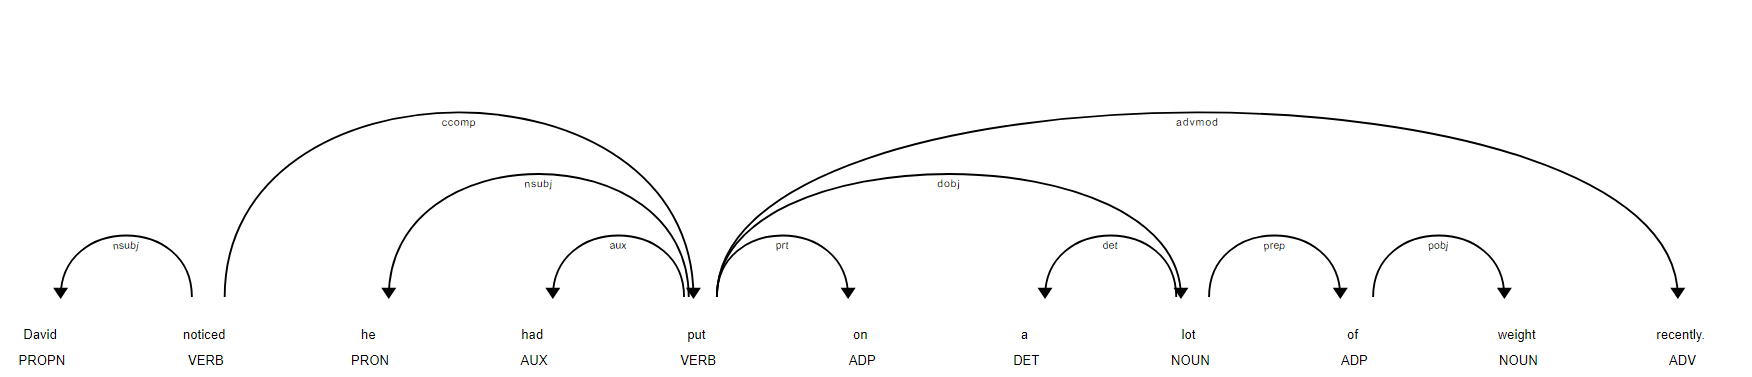
\includegraphics[width=8cm]{spacy.png}};
    \end{tikzpicture}
    \caption{Spacy Dependency Example}
\end{figure}

Using SPACY, we parse through all our sentences capturing words that are labeled ``ROOT" (for verb), ``nsubj" (for subject), or ``dobj"/``pobj" (for object) 
into our SVO triples. It is important to note that ``ROOT" can be a successful tag for verbs, but isn't a guarantee. As noted in Figure 1, certain words 
such as ``put" are stronger central nodes than others since they share more dependencies.  This will be important to improve upon to optimally capture 
significant SVOs.

After generating SVOs, one for each story sentence, we use a bert model to generate cosine similarities for our different endings. We do so by
tokenizing our SVOs then running them through a bert model to obtain a mean pooled output for each triple. The story endings are treated the same.
Next we compute a cosine similarity between all the story sentences and the two possible endings (Figure 2). The initial attempt to use triples hasn't yieled
 remarkable results, only presenting a 50 percent accuracy.

\begin{figure}[H]
    \centering
    \begin{tikzpicture}
        \node at (0,0) {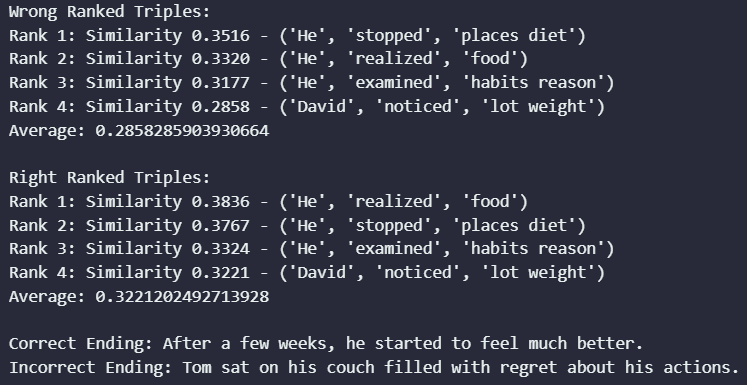
\includegraphics[width=8cm]{Cosine_Similarity.png}};
    \end{tikzpicture}
    \caption{Consine Similarity}
\end{figure}

However, the next models will investigate triples with better selection and ordering of the triples. Currently, all triples are weighed evenly 
when the cosines are averaged (Figure 2). The next model iteration will note the ending triples of the story more using a BertSeqtoSeq model. 

\end{multicols}

\end{document}

